% !TeX program = xelatex
\documentclass[UTF8,a4paper,12pt,fontset=fandol]{ctexart}
\usepackage[left=3.18cm,right=3.18cm,top=2.54cm,bottom=2.54cm]{geometry}
\usepackage{amsmath,amssymb,booktabs,graphicx,caption,xcolor,tabularx,listings,xurl,tikz}
\usepackage[hidelinks]{hyperref}
\usepackage{bookmark}
\usepackage{placeins}
\usetikzlibrary{arrows.meta}
\definecolor{inkblue}{HTML}{235B8E}
\hypersetup{pdftitle={自由基异构化反应的机理研究},pdfauthor={叶青杨}}
\graphicspath{{figures/}}
\captionsetup{font=small,labelfont=bf,skip=5pt}
\setlength{\parindent}{2em}
\setlength{\parskip}{3pt}
\renewcommand{\arraystretch}{1.18}
\pagestyle{plain}
\ctexset{section={format=\sffamily\large\bfseries\raggedright,beforeskip=.9em,afterskip=.45em},
 subsection={format=\sffamily\normalsize\bfseries\raggedright,beforeskip=.7em,afterskip=.3em}}
\renewcommand{\topfraction}{.9}
\renewcommand{\bottomfraction}{.85}
\renewcommand{\textfraction}{.08}
\renewcommand{\floatpagefraction}{.75}
\setlength{\emergencystretch}{2em}
\definecolor{codebg}{RGB}{244,246,248}
\lstset{basicstyle=\ttfamily\footnotesize,backgroundcolor=\color{codebg},breaklines=true,
 columns=fullflexible,keepspaces=true,frame=single,rulecolor=\color{codebg},showstringspaces=false}
\newcommand{\kcal}{\mathrm{kcal\,mol^{-1}}}
\newcommand{\Eh}{E_{\mathrm h}}
\begin{document}
\begin{titlepage}
\centering\vspace*{1cm}
{\fontsize{24pt}{36pt}\selectfont\bfseries 浙江大学量子化学实验\par}
\vspace{1cm}
{\sffamily\fontsize{18pt}{24pt}\selectfont 自由基异构化反应的机理研究\par}
\vspace{.7cm}
{\sffamily\fontsize{22pt}{28pt}\selectfont\bfseries 实\\[.32cm]验\\[.32cm]报\\[.32cm]告\par}
\vfill
{\fontsize{14pt}{21pt}\selectfont 参加学生：叶青杨\par}
\vspace{1cm}
{\fontsize{18pt}{24pt}\selectfont\bfseries 浙江大学化学实验教学中心\par}
\vspace{.5cm}
{\fontsize{18pt}{24pt}\selectfont\bfseries 2026年10月19日\par}
\end{titlepage}
\setcounter{page}{1}\fontsize{12pt}{18pt}\selectfont
\begin{center}
{\sffamily\fontsize{15pt}{22pt}\selectfont\bfseries 自由基异构化反应的机理研究\par}
\vspace{.4em}叶青杨
\end{center}

\noindent\textbf{摘要}\quad
采用 UB3LYP-D3(BJ)/def2-SVP 方法研究环丙基甲基自由基开环为
3-丁烯-1-基自由基的过程。过渡态具有唯一的 $626.12i\ \mathrm{cm^{-1}}$
开环振动，双向 IRC 连接环状反应物与开链产物。
电子活化能为 $8.89\ \kcal$；在 298.15 K、1 atm 下，
活化 Gibbs 自由能为 $8.35\ \kcal$，反应自由能为 $-3.35\ \kcal$。
随着 C1--C2 断裂和 C2=C9 形成，主要自旋布居由 C9 转移至 C1。
固定相同几何的 DLPNO-CCSD(T1)/def2-TZVPP 电子势垒为 $8.94\ \kcal$；
B3LYP-D3(BJ) 扩展基组后为 $7.42\ \kcal$，M06-2X 为 $12.41\ \kcal$，
显示电子势垒与反应能对方法和基组的依赖。

\section{实验目的}
以课件中的环丙基甲基自由基开环为对象，掌握开壳层体系的电子数、自旋多重度和非限制性波函数设置，
通过柔性扫描、过渡态优化与 IRC 建立反应通道。
结合沿途自旋布居、真实自旋密度与驻点热化学，解释断键、成键和未配对电子重新分布的关系，
并用独立理论结果对照关键能垒\cite{course}。

\section{实验原理与计算方法}
\subsection{体系、电子态与共同原子编号}
体系为中性 C$_4$H$_7$ 自由基，含 11 个原子和 31 个电子，
$N_\alpha=16$、$N_\beta=15$，总自旋 $S=1/2$。
采用非限制性 Kohn--Sham 描述，使 $\alpha$ 与 $\beta$ 电子可以占据不同的空间轨道，表达自由基的自旋极化。
所有结构保留课件的共同编号：C1、C2、C3、H4--H8、C9、H10、H11。
反应物的三元环为 C1--C2--C3，C9 是环外自由基碳；
产物碳链为 C1--C3--C2=C9，末端 C1 为主要自由基中心。

\begin{figure}[htbp]
\centering
\begin{tikzpicture}[font=\small,line width=.8pt]
\node (a) at (0,0) {C1H$_2$};\node (b) at (1.2,1.0) {C2H};
\node (c) at (2.4,0) {C3H$_2$};\node (d) at (1.2,2.0) {$\boldsymbol{\cdot}$C9H$_2$};
\draw (a)--(b)--(c)--(a);\draw (b)--(d);
\draw[-{Stealth[length=2.5mm]}] (3.1,.8)--(4.2,.8);
\node (e) at (5.0,.8) {$\boldsymbol{\cdot}$C1H$_2$};\node (f) at (6.5,.8) {C3H$_2$};
\node (g) at (7.9,.8) {C2H};\node (h) at (9.3,.8) {C9H$_2$};
\draw (e)--(f)--(g);\draw[double,double distance=2pt] (g)--(h);
\node at (1.2,-.6) {环状自由基 R};\node at (7.1,-.6) {开链自由基 P};
\end{tikzpicture}
\caption{开环反应及共同碳编号。自由基点表示主要自旋位置，计算中的全部氢编号保持不变。}
\end{figure}

\subsection{约束扫描、驻点与反应通道}
柔性扫描在给定 C1--C2 距离下优化其他自由度，扫描峰用于定位初猜。
无约束驻点满足 $\nabla E=0$；在质量加权坐标 $Q$ 下，局部势能展开为
\begin{equation}
E(Q)\simeq E_0+\tfrac12 Q^{\mathrm T}H_{\rm mw}Q,
\qquad H_{\rm mw}=M^{-1/2}HM^{-1/2}.
\end{equation}
扣除整体平移、转动后，本体系有 $3N-6=27$ 个振动自由度。
极小值的振动曲率均为正，一阶鞍点有一个负本征值，表现为唯一虚频。
虚频位移识别局部反应运动，IRC 从鞍点沿质量加权最陡下降方向追踪，确定两侧连接的极小值\cite{irc}。

\subsection{电子结构与热化学设置}

首先用 UPM7 对 C1--C2 距离作柔性扫描，每次递增 0.1 \AA，
其余自由度放松。以开环区间的局部能量峰为初猜，在
Gaussian 16 中进行 UB3LYP-D3(BJ)/def2-SVP 过渡态优化与解析频率计算。
DFT 计算统一采用 \texttt{SCF=(Tight,XQC)}、\texttt{Int=UltraFine}、
\texttt{NoSymm}，气相、中性双重态。
反应物、过渡态和产物均作波函数稳定性检验。
主要过渡态输入为
\begin{lstlisting}
#p UB3LYP/Def2SVP EmpiricalDispersion=GD3BJ
   SCF=(Tight,XQC) Int=UltraFine NoSymm
   Opt=(TS,CalcFC,NoEigenTest,Tight,MaxCycles=200) Freq
\end{lstlisting}
\texttt{CalcFC} 在初始几何计算 Hessian；\texttt{NoEigenTest} 不取消最终频率与虚频运动的检验。

IRC 分别沿过渡态虚频的两个方向追踪，设置为
\begin{lstlisting}
IRC=(Forward,CalcFC,ReCalc=3,StepSize=5,MaxPoints=50)
IRC=(Reverse,CalcFC,ReCalc=3,StepSize=5,MaxPoints=50)
\end{lstlisting}
其中 \texttt{StepSize=5} 按 Gaussian 百分之一单位约定取 0.05，
路径图使用程序输出的质量加权坐标 $q$（$\sqrt{\mathrm{amu}}\,a_0$）\cite{irc}。
两端进一步无约束优化并计算频率；热化学采用
298.15 K、1 atm 的刚性转子--谐振子（RRHO）近似，频率不缩放\cite{thermo}。
各驻点都是双重态，电子自旋简并贡献在差值中相消；转动对称数分别审计。
过渡态的虚频不作为稳定谐振动计入配分函数。

另在上述 R、TS、P 几何上作三组独立电子能对照：
UB3LYP-D3(BJ)/def2-TZVPP、UM06-2X/def2-TZVPP 和
DLPNO-CCSD(T1)/def2-TZVPP。
前两组采用球谐基函数（222 个）、UltraFine 网格，并分别检验波函数稳定性。
M06-2X 不额外叠加色散修正；def2-TZVPP 提供三重 $\zeta$ 价层及双极化描述\cite{m06,def2}。
耦合簇采用 UHF 导出的准限制轨道（QRO）、TightPNO、匹配的 def2-TZVPP/C 辅助基组，
冻结 8 个化学内层电子，并包含迭代三激发修正\cite{mdci}。
这些对照均固定原子坐标，只比较各自方法内部的电子能差。

\begin{figure}[h!]
\centering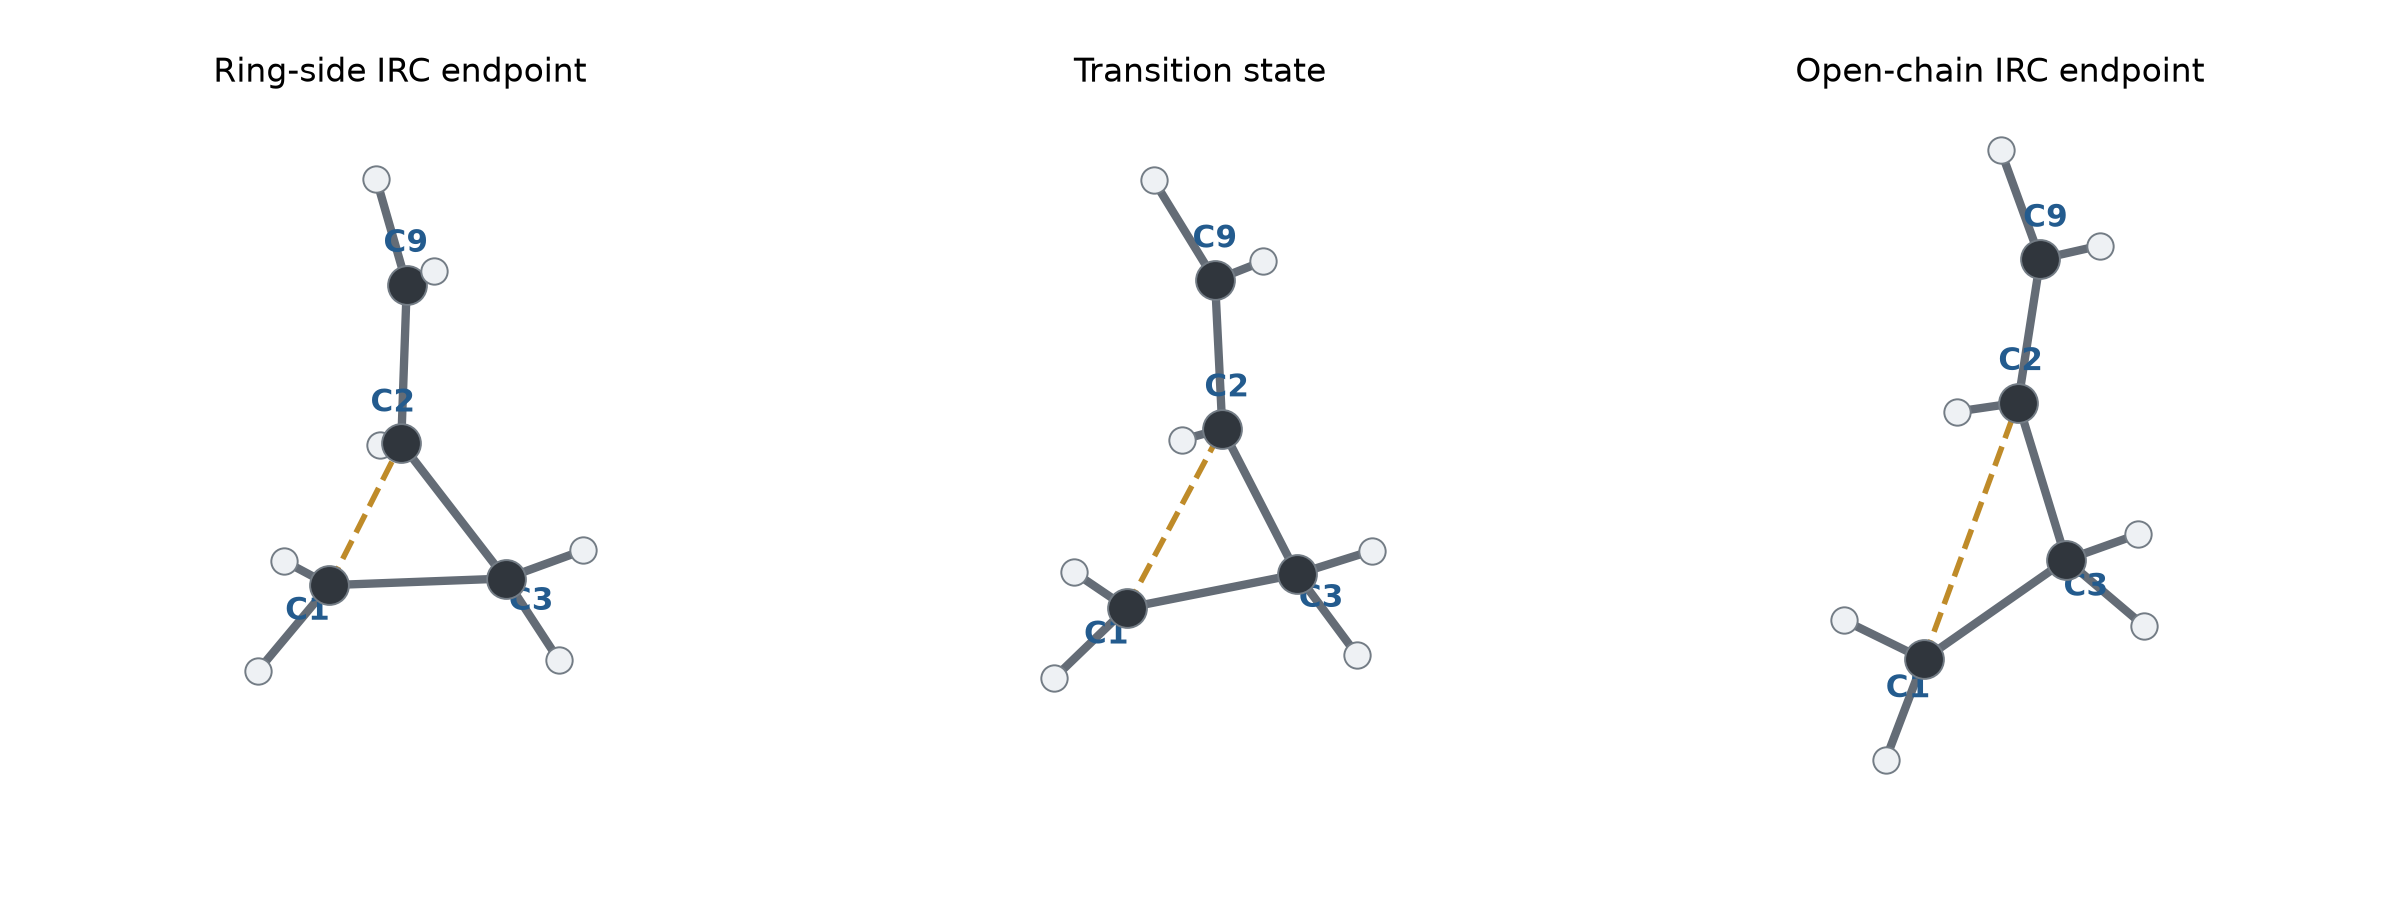
\includegraphics[width=\linewidth]{irc-key-geometries.png}
\caption{IRC 两端与过渡态的共同原子编号。虚线标出逐渐断裂的 C1--C2；
右侧 C2--C9 在开环过程中缩短。两端图示为 IRC 末点，驻点能量取进一步优化后的极小值。}
\end{figure}

\section{柔性扫描与过渡态}
\subsection{开环峰与未收敛尾部的处理}
初次扫描的 16 个位置中，1.51--2.51 \AA{} 的 11 点收敛；
尾部五点经调整几何优化算法后全部收敛，形成完整的 1.51--3.01 \AA{} 柔性扫描。
开环区间的局部峰位于 1.91 \AA，
相对首个约束结构高 $7.59\ \kcal$，据此获得 DFT 过渡态初猜。
该 PM7 扫描用于定位初猜，最终能垒取无约束 DFT 驻点之差。

未收敛尾部的 SCF 已收敛，问题出在几何优化。
最后 20 步显示近似二周期振荡：C2--C9 在相邻两步间变化约 0.02646 \AA，
隔两步则几乎重复；五点末态最大力为 $0.00928$--$0.03161\ \Eh\,a_0^{-1}$，
高于 $0.00045\ \Eh\,a_0^{-1}$ 的收敛阈值。
因此修复保持 UPM7 和原收敛阈值，采用每步重算 Hessian 的
\texttt{CalcAll}、较小初始步长 \texttt{MaxStep=1}，每点最多 200 步\cite{opt}。
2.61 \AA{} 试点的四项几何判据全部通过，最大力降至
$10^{-6}\ \Eh\,a_0^{-1}$，同样设置随后使 2.71--3.01 \AA{} 的四点收敛。
试点与后续扫描在 2.61 \AA{} 的重叠结构能量一致。

完整曲线在约 2.51 \AA{} 的开链区域达到低能点，随后随强制增大 C1--C2 距离再次上升，
3.01 \AA{} 处相对初始结构高 $17.78\ \kcal$。
这段对应开链骨架被进一步拉伸，并非另一条经无约束鞍点确认的反应通道。
例如，在 3.01 \AA{} 约束处，C1--C3、C2--C3 分别增至 1.577、1.650 \AA，
同时 $\angle$C1--C3--C2 增至 $137.74^\circ$。
因此寻找开环 TS 时应选 1.91 \AA{} 的局部峰，而不是扫描末端的全局最高能量。

\begin{figure}[h!]
\centering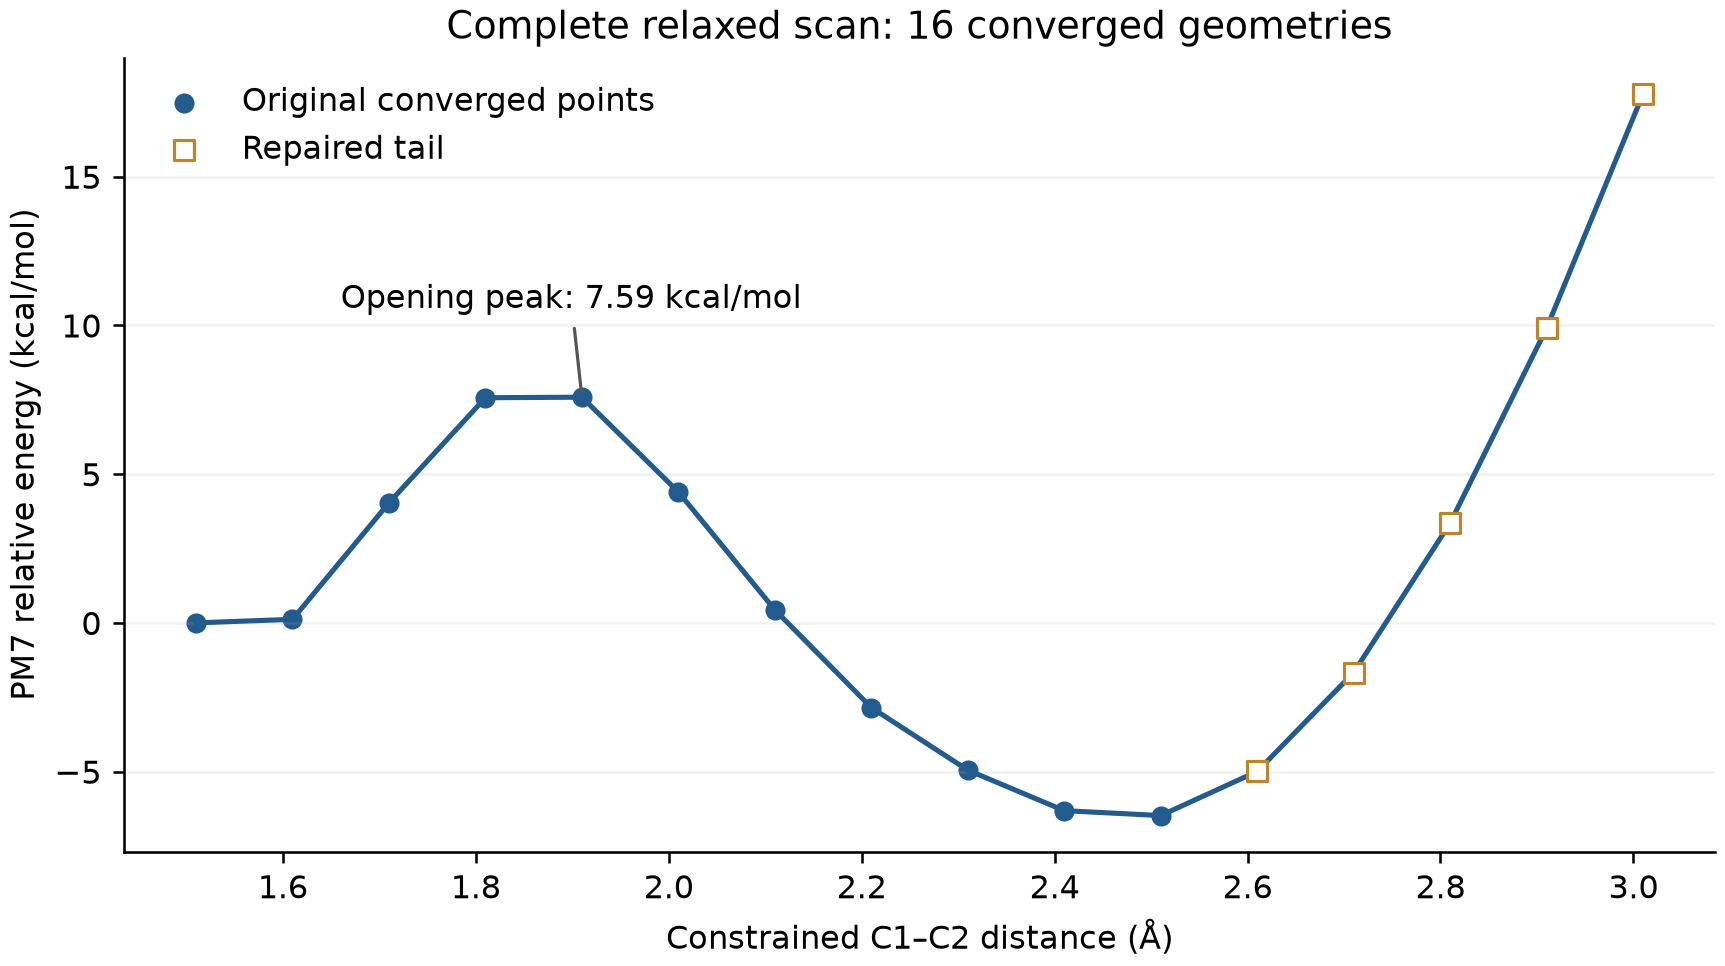
\includegraphics[width=.92\linewidth]{pm7-scan-complete.png}
\caption{完整 UPM7 柔性扫描。圆点为原始收敛点，空心方块为修复后收敛的尾部。
能量以 1.51 \AA{} 的约束结构为零点；全部点保持相同方法和收敛阈值。}
\end{figure}

\subsection{唯一虚频与关键键长}
DFT 过渡态的 27 个振动中只有一个虚频，数值为
$626.12i\ \mathrm{cm^{-1}}$。位移表现为 C1--C2 拉长，同时 C2--C9 缩短，
与目标开环和双键形成一致。其余 26 个振动均为实频。
该结构的最大 Cartesian 梯度分量为 $1.88\times10^{-6}\ \Eh\,a_0^{-1}$。

\begin{figure}[htbp]
\centering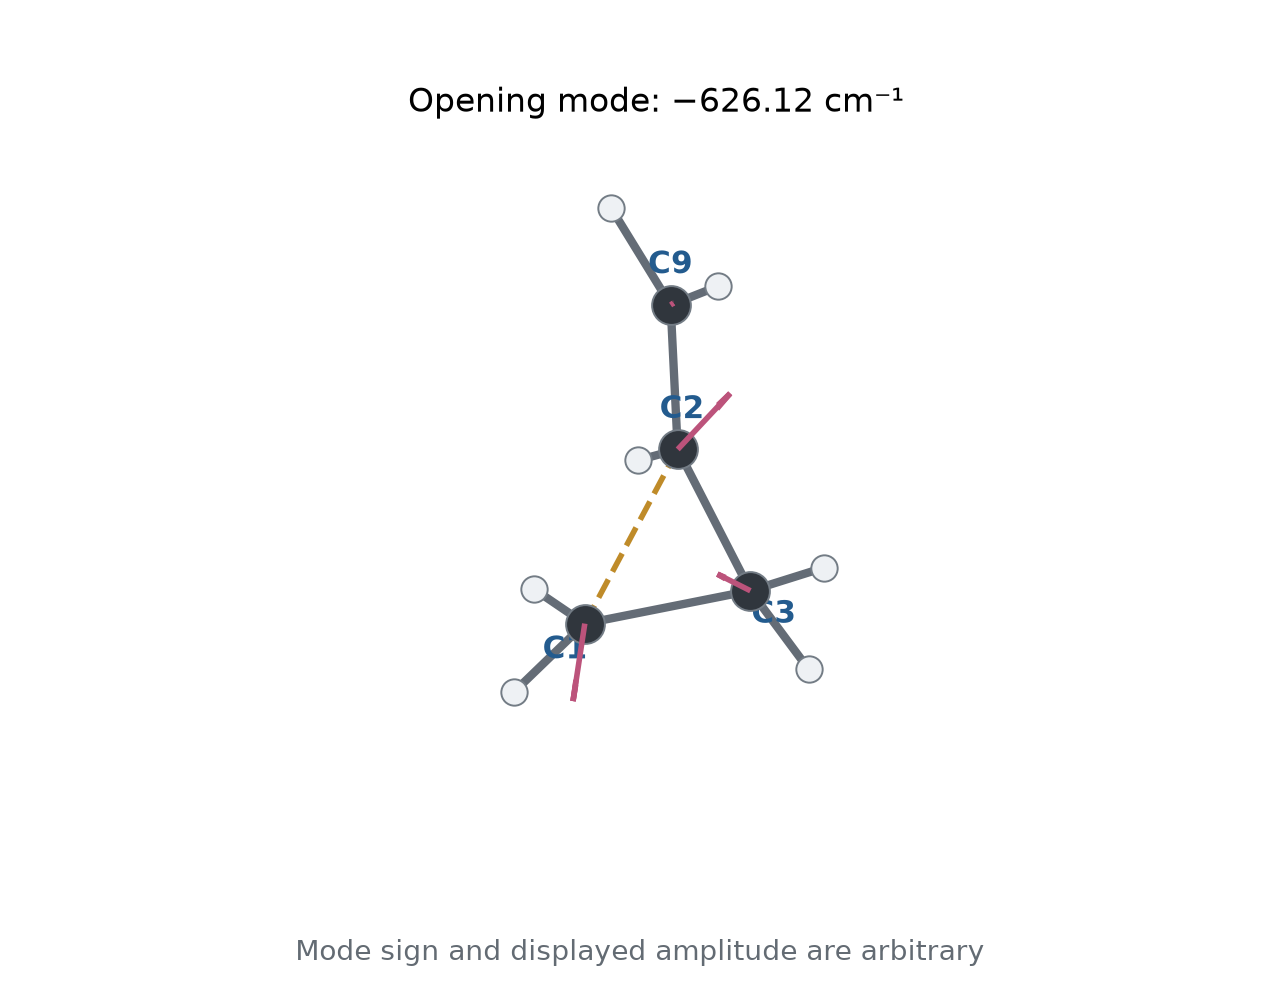
\includegraphics[width=.56\linewidth]{ts-opening-mode.png}
\caption{过渡态开环振动。箭头表示真实虚频位移，正负方向等价。}
\end{figure}
\begin{table}[htbp]
\centering\caption{驻点的关键键长（\AA）}
\begin{tabular}{lrrr}\toprule
键 & R & TS & P\\\midrule
C1--C2 & 1.531 & 1.917 & 2.508\\
C1--C3 & 1.494 & 1.482 & 1.494\\
C2--C3 & 1.531 & 1.495 & 1.507\\
C2--C9 & 1.458 & 1.386 & 1.335\\\bottomrule
\end{tabular}
\end{table}
C1--C2 从三元环中的共价键发展为非键接触，C2--C9 则达到典型双键长度。
C1--C3 和 C2--C3 保持成键，构成开链产物的骨架。
TS 中断裂键已显著伸长，C2--C9 处于单双键长度之间，说明断环和双键形成共同参与过渡结构。

\section{IRC 连通性与沿途电子结构}
\subsection{双向路径与端点身份}
正向 IRC 得到 38 个非 TS 接受点，通向开链侧；反向得到 17 点，
通向环状侧，两侧均检测到势能面极小值区域。
将两端继续优化后均得到 27 个实频。
反向端点与独立优化的反应物经等价氢映射和正旋转配准后，
全原子 RMSD 为 $3.70\times10^{-5}$ \AA，确认回到同一反应物。
正向端点为 C1--C3--C2=C9 开链自由基。

\begin{figure}[htbp]
\centering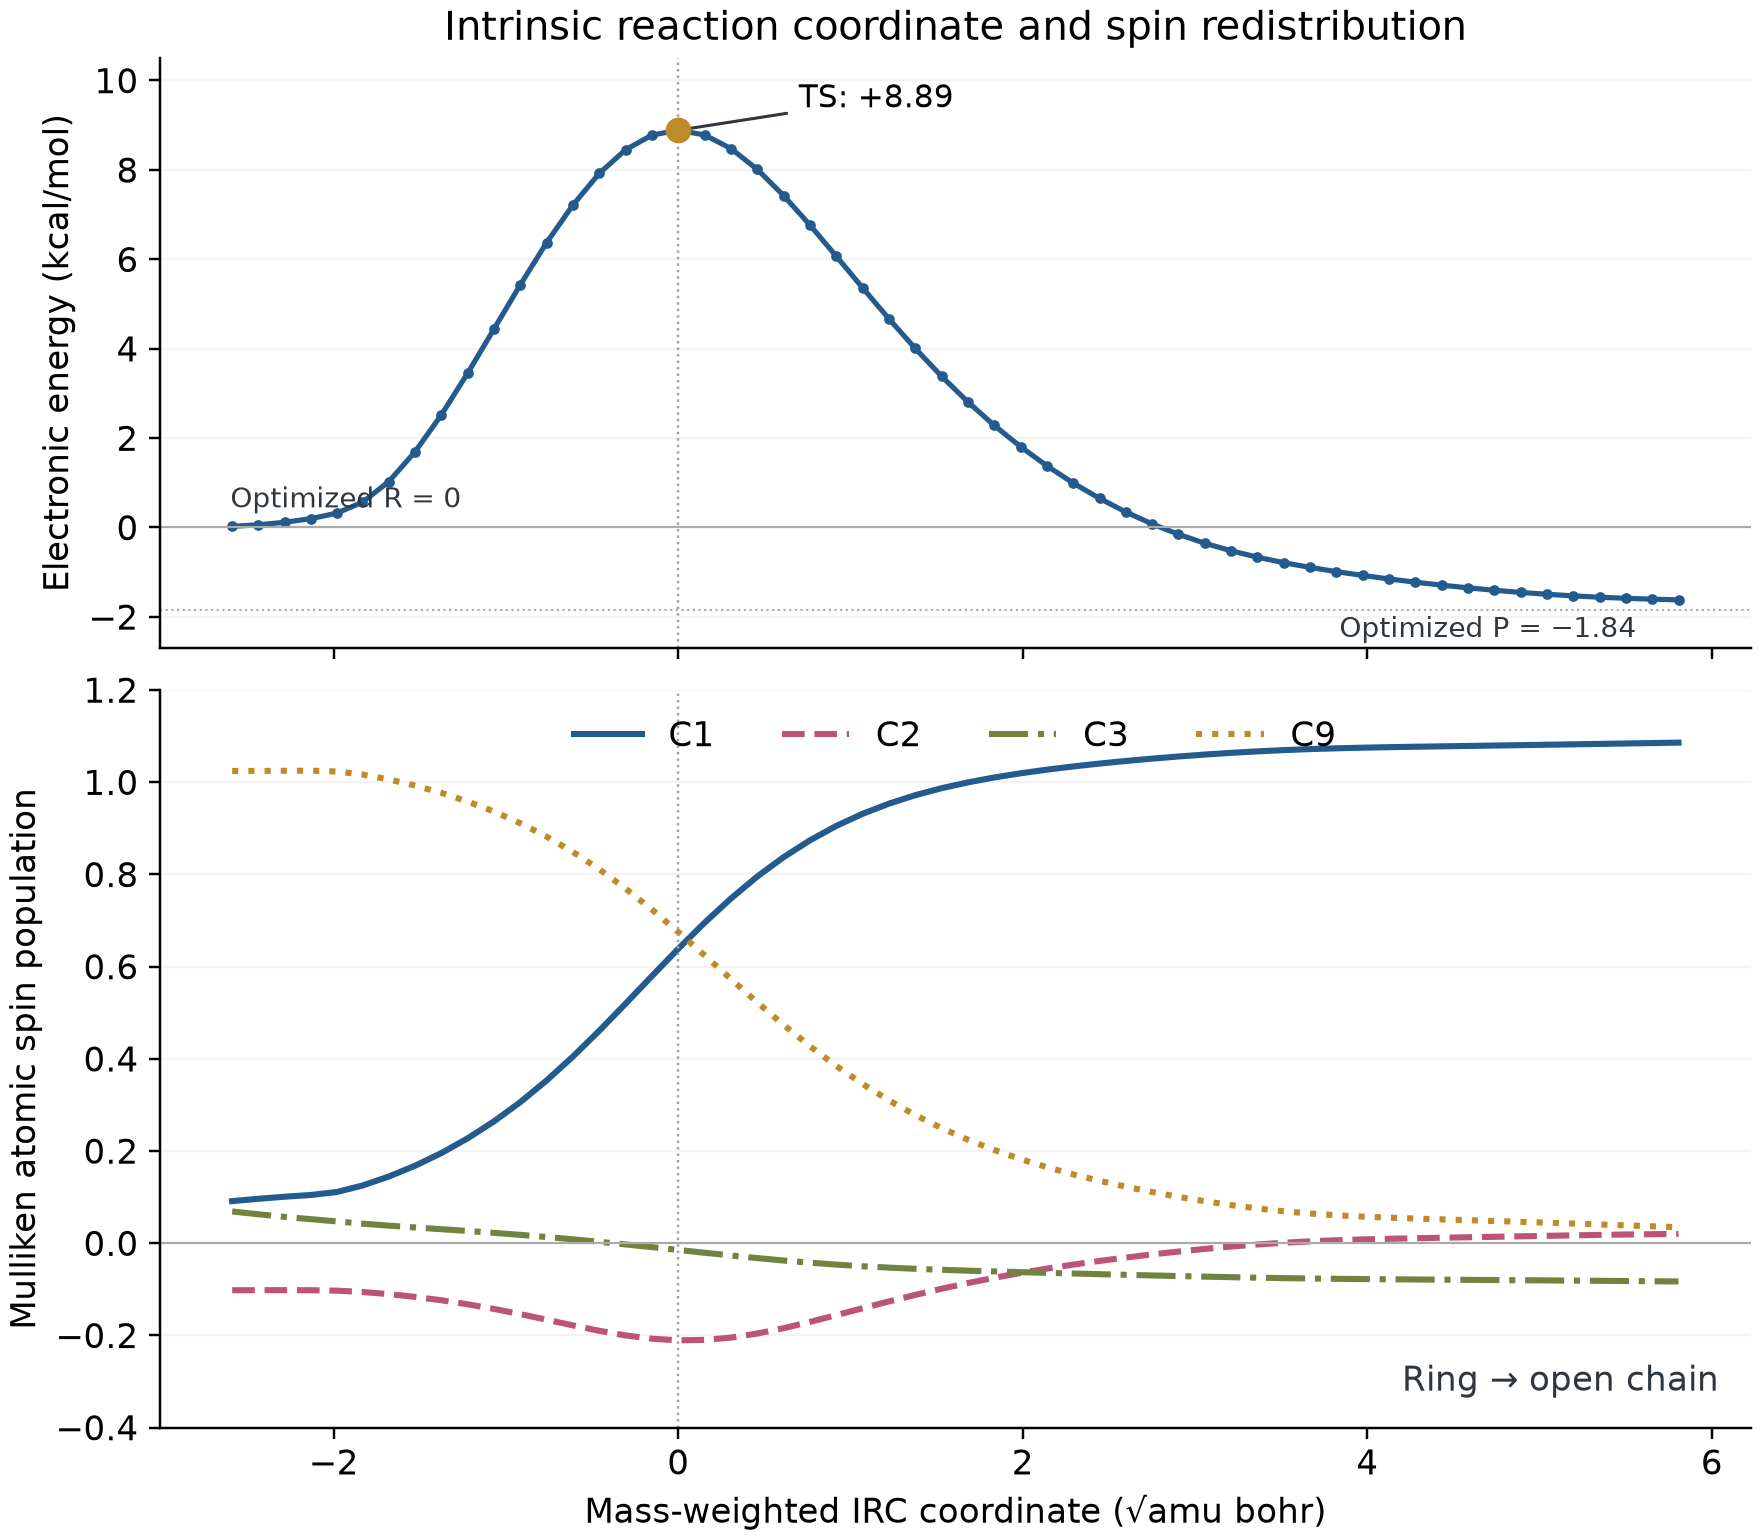
\includegraphics[width=.97\linewidth]{irc-energy-spin.png}
\caption{56 个不同接受结构（含一次 TS）的 IRC 电子能及碳原子自旋布居。
能量与布居均在对应结构上以同一 DFT 方法求得，能量零点为优化反应物 R。
虚线水平线标出优化产物能量；曲线末点随后继续优化，因而与该水平线略有差别。}
\end{figure}

\noindent
路径能量从 TS 向两侧下降，未出现第二个极大值或中间极小值。
C9 自旋随开环连续减小，C1 自旋连续增大；过渡态附近两者接近，
表明结构重组与自旋重新分配发生在同一反应步骤中。

\subsection{键长变化与波函数的连续性}
图~\ref{fig:bondpath} 将四条关键碳间距离放在同一反应坐标上比较。
C1--C2 的主要伸长与 C2--C9 的主要缩短集中在 TS 周围，
而保留的 C1--C3、C2--C3 只作小幅调整。
因此所追踪通道是单步开环重排，不含先断环、再另行成双键的长寿命中间体。
结构变化与自旋迁移来自同一组接受结构；横坐标描述势能面上的路径，不代表真实时间。
\begin{figure}[htbp]
\centering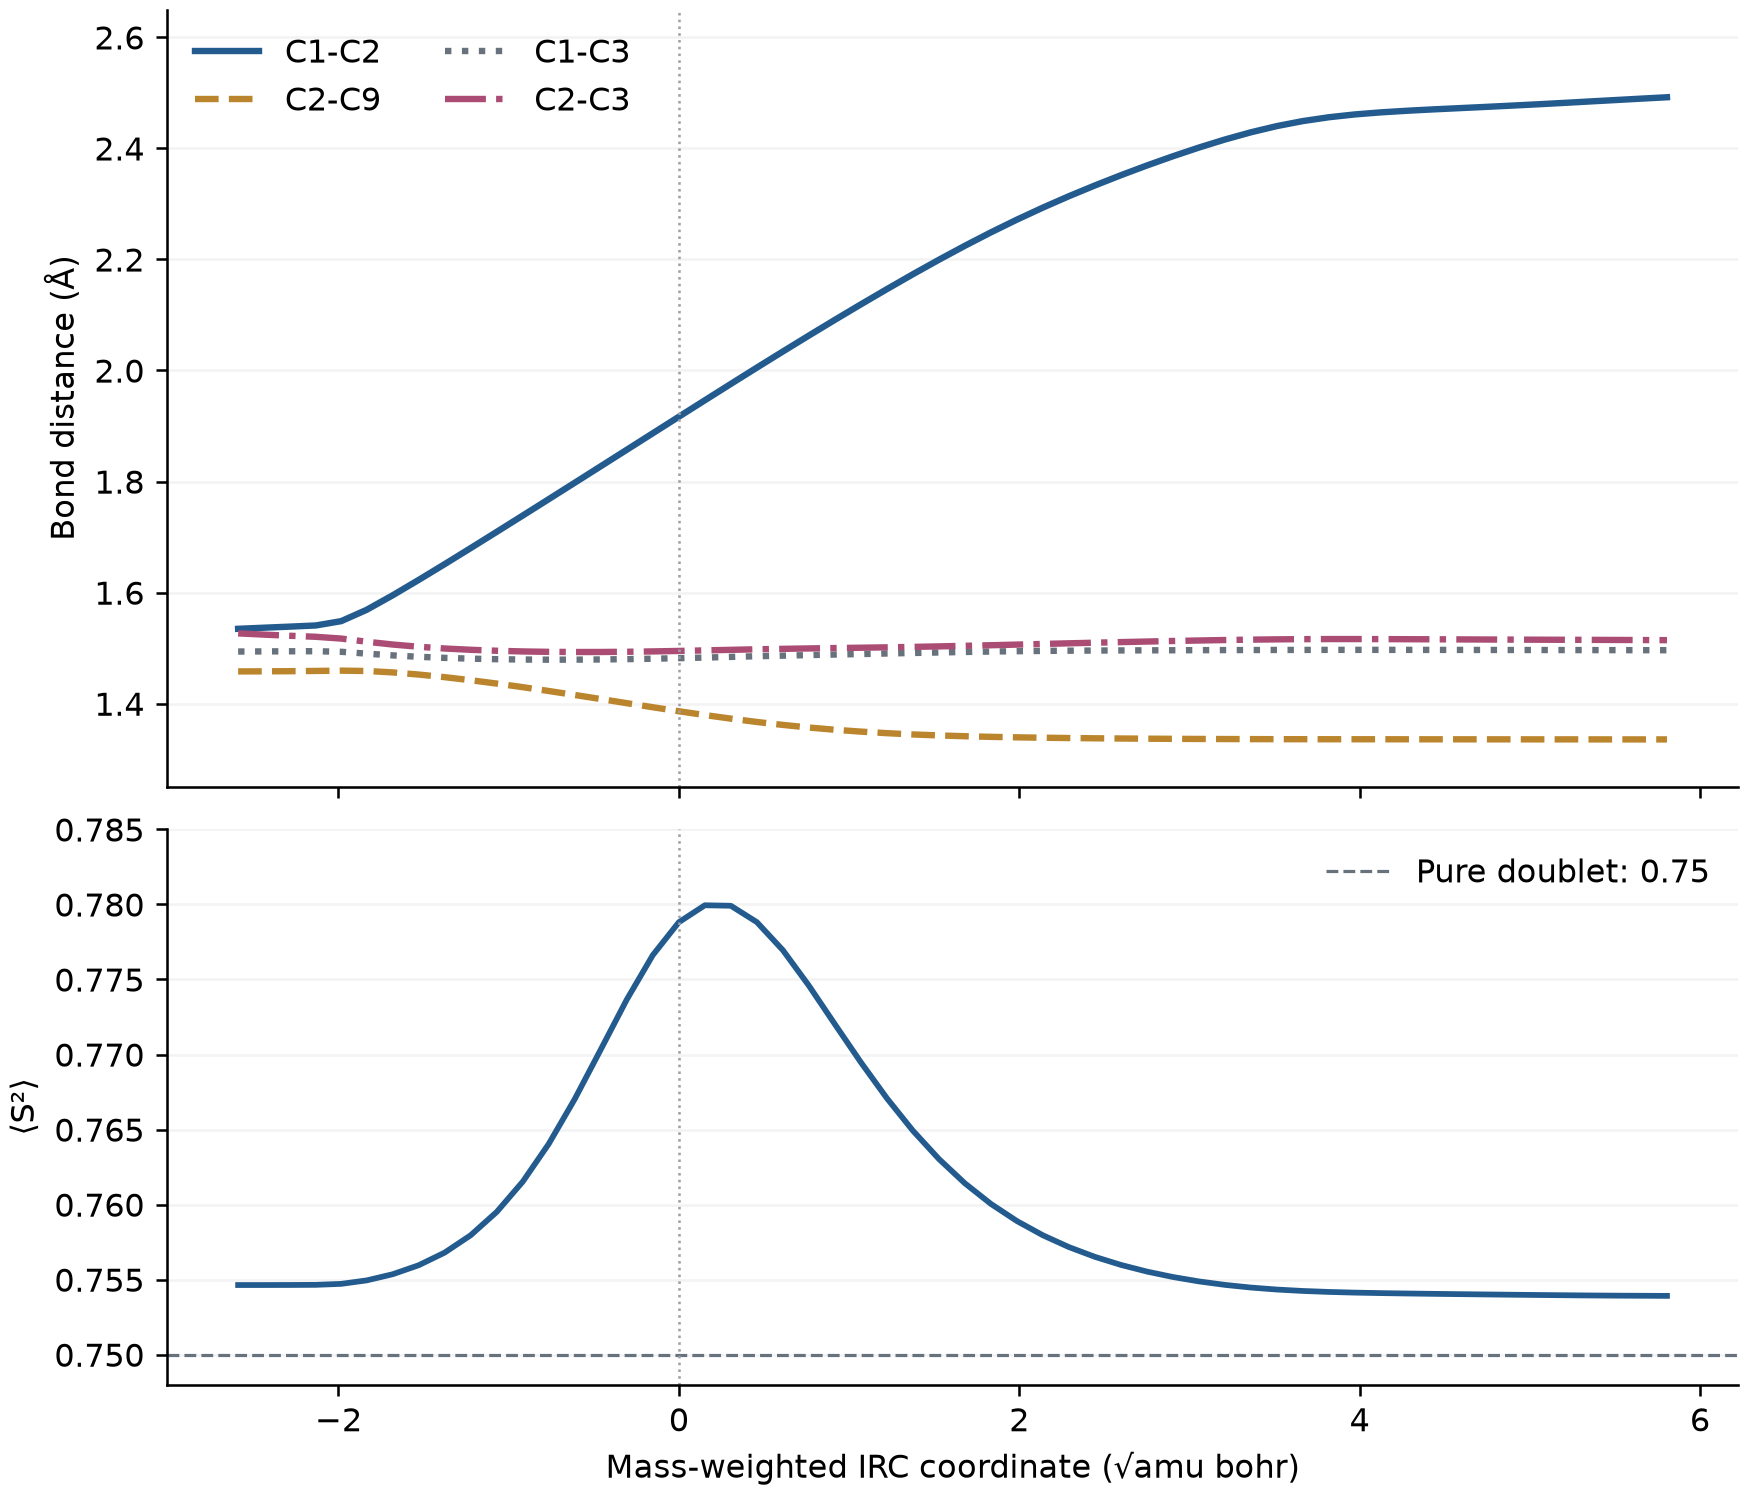
\includegraphics[width=.91\linewidth]{irc-bond-spinquality.png}
\caption{沿 IRC 的关键碳间距离与 $\langle S^2\rangle$。竖线为 TS，水平虚线为理想双重态值 0.75。}
\label{fig:bondpath}
\end{figure}

\section{自旋布居、自旋密度与波函数}
\subsection{原子布居与真实空间密度}
反应物 C9 的 Mulliken 自旋布居为 1.024，产物 C1 为 1.087。
过渡态的 C1 和 C9 分别为 0.639 和 0.675，显示两个部位共同承载主要自旋。
原子自旋布居是 $\alpha$ 与 $\beta$ 布居之差；邻近原子的负值反映自旋极化，
因此单个原子的值可以略大于 1。全体系布居之和为 1。
56 个 IRC 点的布居求和偏差不超过 $2\times10^{-6}$。
Mulliken 数值依赖基组和分区定义，本实验主要利用同一方法下的沿途变化趋势。
空间自旋密度满足
\begin{equation}
\rho_s(\mathbf r)=\rho_\alpha(\mathbf r)-\rho_\beta(\mathbf r),
\qquad \int\rho_s(\mathbf r)\,\mathrm d\mathbf r=N_\alpha-N_\beta=1.
\end{equation}

\begin{figure}[h!]
\centering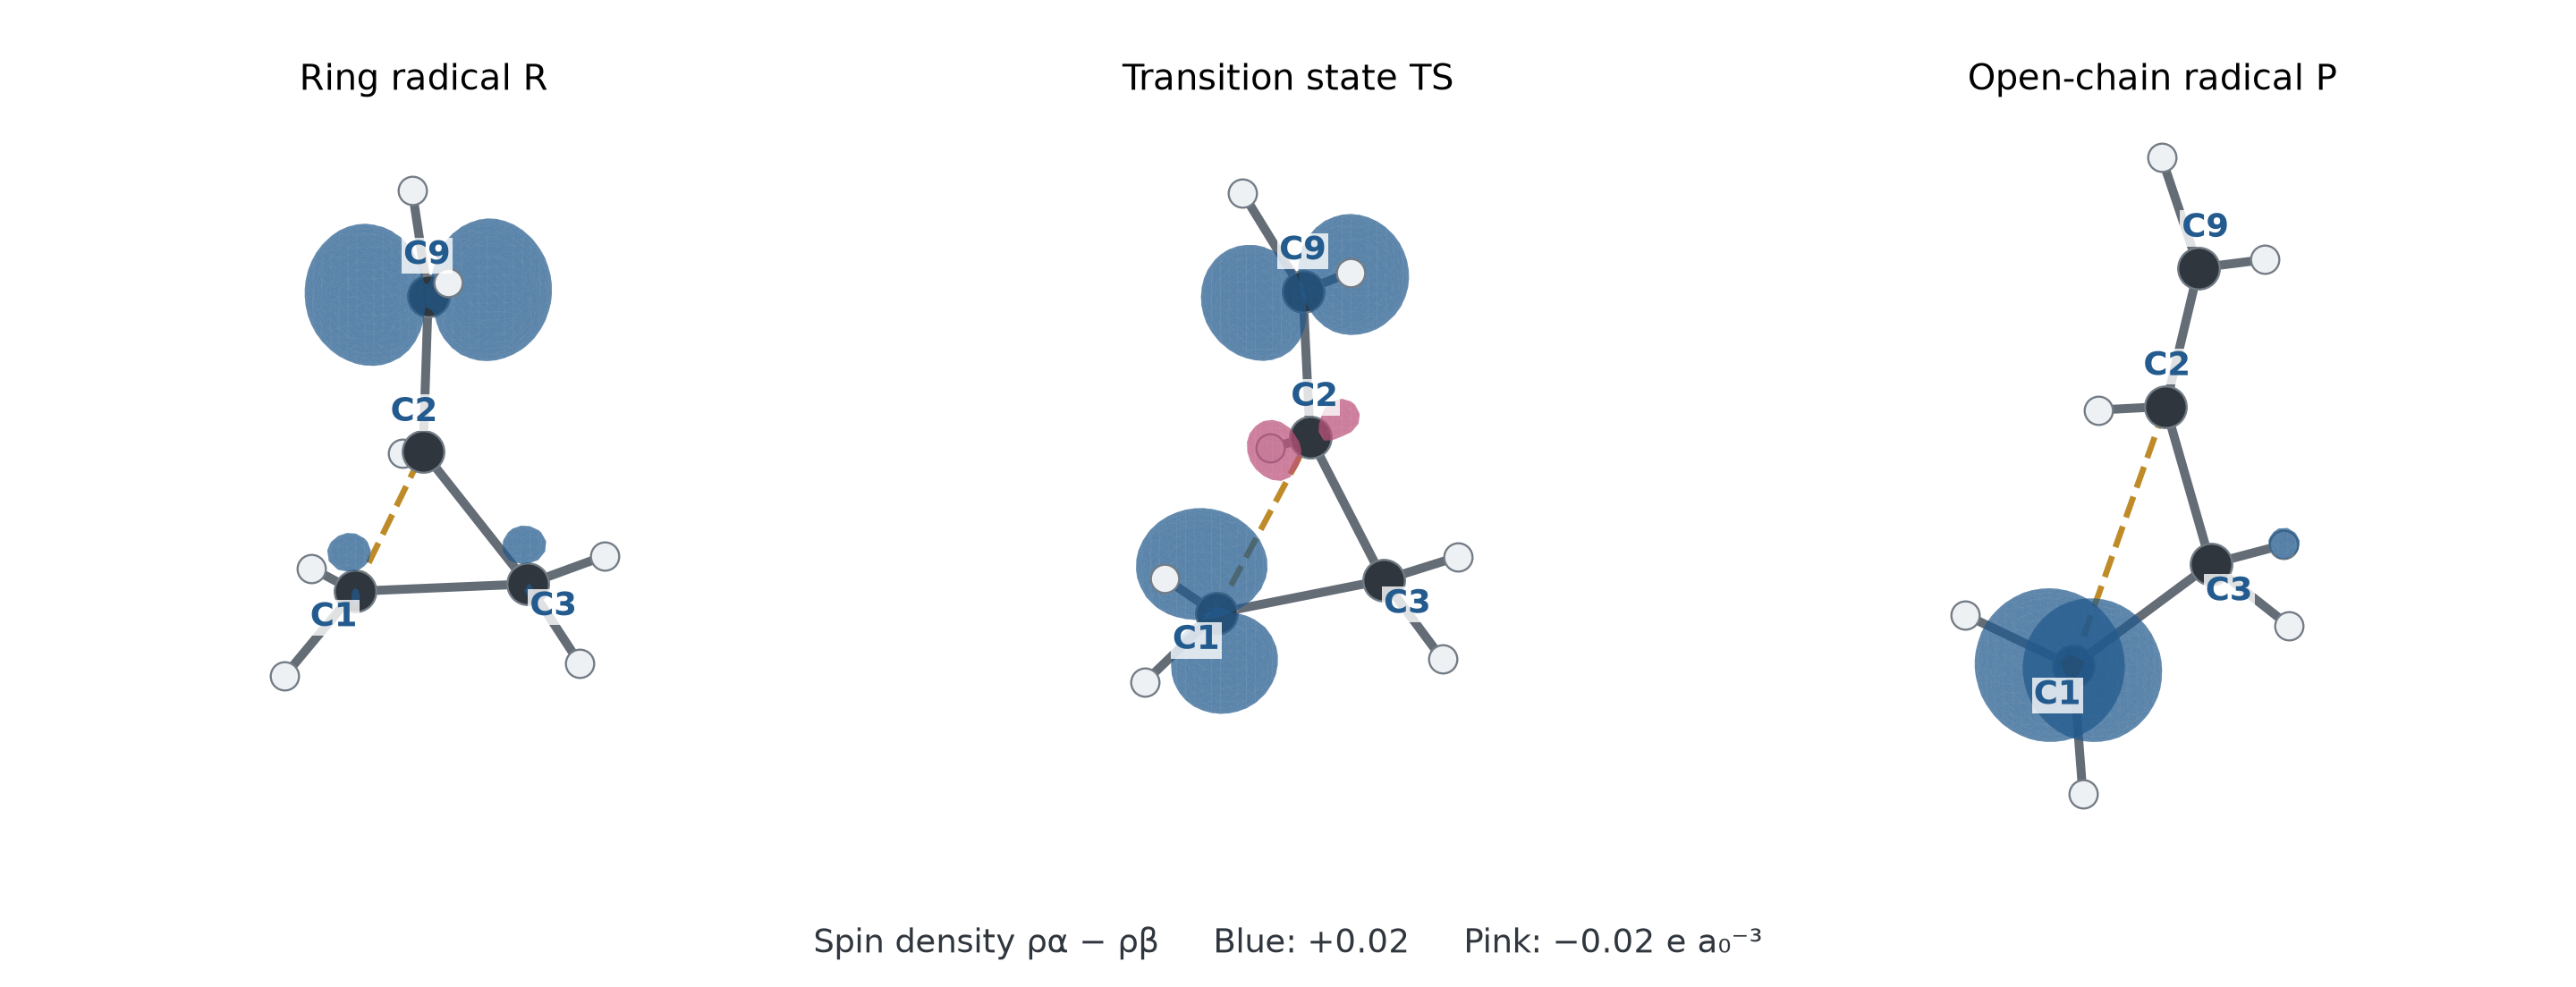
\includegraphics[width=\linewidth]{spin-density.png}
\caption{从 R、TS、P 的波函数得到的 $\rho_\alpha-\rho_\beta$ 等值面。
蓝色为 $+0.02$，粉色为 $-0.02\ e\,a_0^{-3}$。
反应物正自旋主要集中在 C9 的 p 型区域，产物转移至 C1，TS 呈两端分布。
R 和 P 的负密度极值分别为 $-0.01870$ 与 $-0.01522\ e\,a_0^{-3}$，
因此在本阈值下仅 TS 出现粉色等值面。}
\end{figure}

\begin{table}[h!]
\centering\caption{主要碳原子的 Mulliken 自旋布居}
\begin{tabular}{lrrrr}\toprule
结构 & C1 & C2 & C3 & C9\\\midrule
R & 0.080 & $-0.102$ & 0.080 & 1.024\\
TS & 0.639 & $-0.211$ & $-0.015$ & 0.675\\
P & 1.087 & 0.010 & $-0.085$ & 0.006\\\bottomrule
\end{tabular}
\end{table}

\subsection{自旋污染与波函数稳定性}
\begin{table}[h!]
\centering\small\caption{波函数与振动特征}
\begin{tabular}{lrrrr}\toprule
结构 & $\langle S^2\rangle$ & 湮灭后 $\langle S^2\rangle$ & 虚频数 & 最低实频/$\mathrm{cm^{-1}}$\\\midrule
R & 0.754644 & 0.750016 & 0 & 162.02\\
TS & 0.778814 & 0.750159 & 1 & 278.69\\
P & 0.753862 & 0.750010 & 0 & 98.79\\\bottomrule
\end{tabular}
\end{table}

理想双重态的 $\langle S^2\rangle=S(S+1)=0.75$。
三处波函数均通过稳定性检验；TS 的自旋污染略大于两端，
但偏离仍较小。IRC 上 $\langle S^2\rangle$ 为 0.753916--0.779945。
自旋密度使用同一网格上的独立 $\alpha$、$\beta$ 密度交叉核对，
并以全空间积分检验未配对电子总量。
R、TS、P 的积分分别为 0.999998、0.999937、1.000063。
自旋污染与波函数不稳定不是同一概念：前者反映非限制性行列式偏离严格自旋本征态，
后者检查轨道扰动能否进一步降低能量\cite{stable}。
本次稳定性检验后能量不变；湮灭后的 $\langle S^2\rangle$ 只是诊断量，
并未对报告中的 DFT 能量作自旋投影修正。

\section{能量与 Gibbs 自由能}
\subsection{驻点能量与正、逆向势垒}
以单个优化环状自由基 R 为零点，定义
$\Delta E^\ddagger=E_{\rm TS}-E_{\rm R}$、
$\Delta_{\rm r}E=E_{\rm P}-E_{\rm R}$；$G$ 的差值采用相同定义。
三处结构的转动对称数均为 1，与热化学输出一致。

\begin{table}[h!]
\centering\caption{驻点电子能与热化学量（Hartree）}
\small\begin{tabular}{lrrrr}\toprule
结构 & $E$ & ZPE & $H_{298.15}$ & $G_{298.15}$\\\midrule
R & $-156.445431918$ & 0.094074 & $-156.345455$ & $-156.378719$\\
TS & $-156.431267896$ & 0.092830 & $-156.332954$ & $-156.365412$\\
P & $-156.448366065$ & 0.092791 & $-156.349005$ & $-156.384061$\\\bottomrule
\end{tabular}
\end{table}

\begin{figure}[h!]
\centering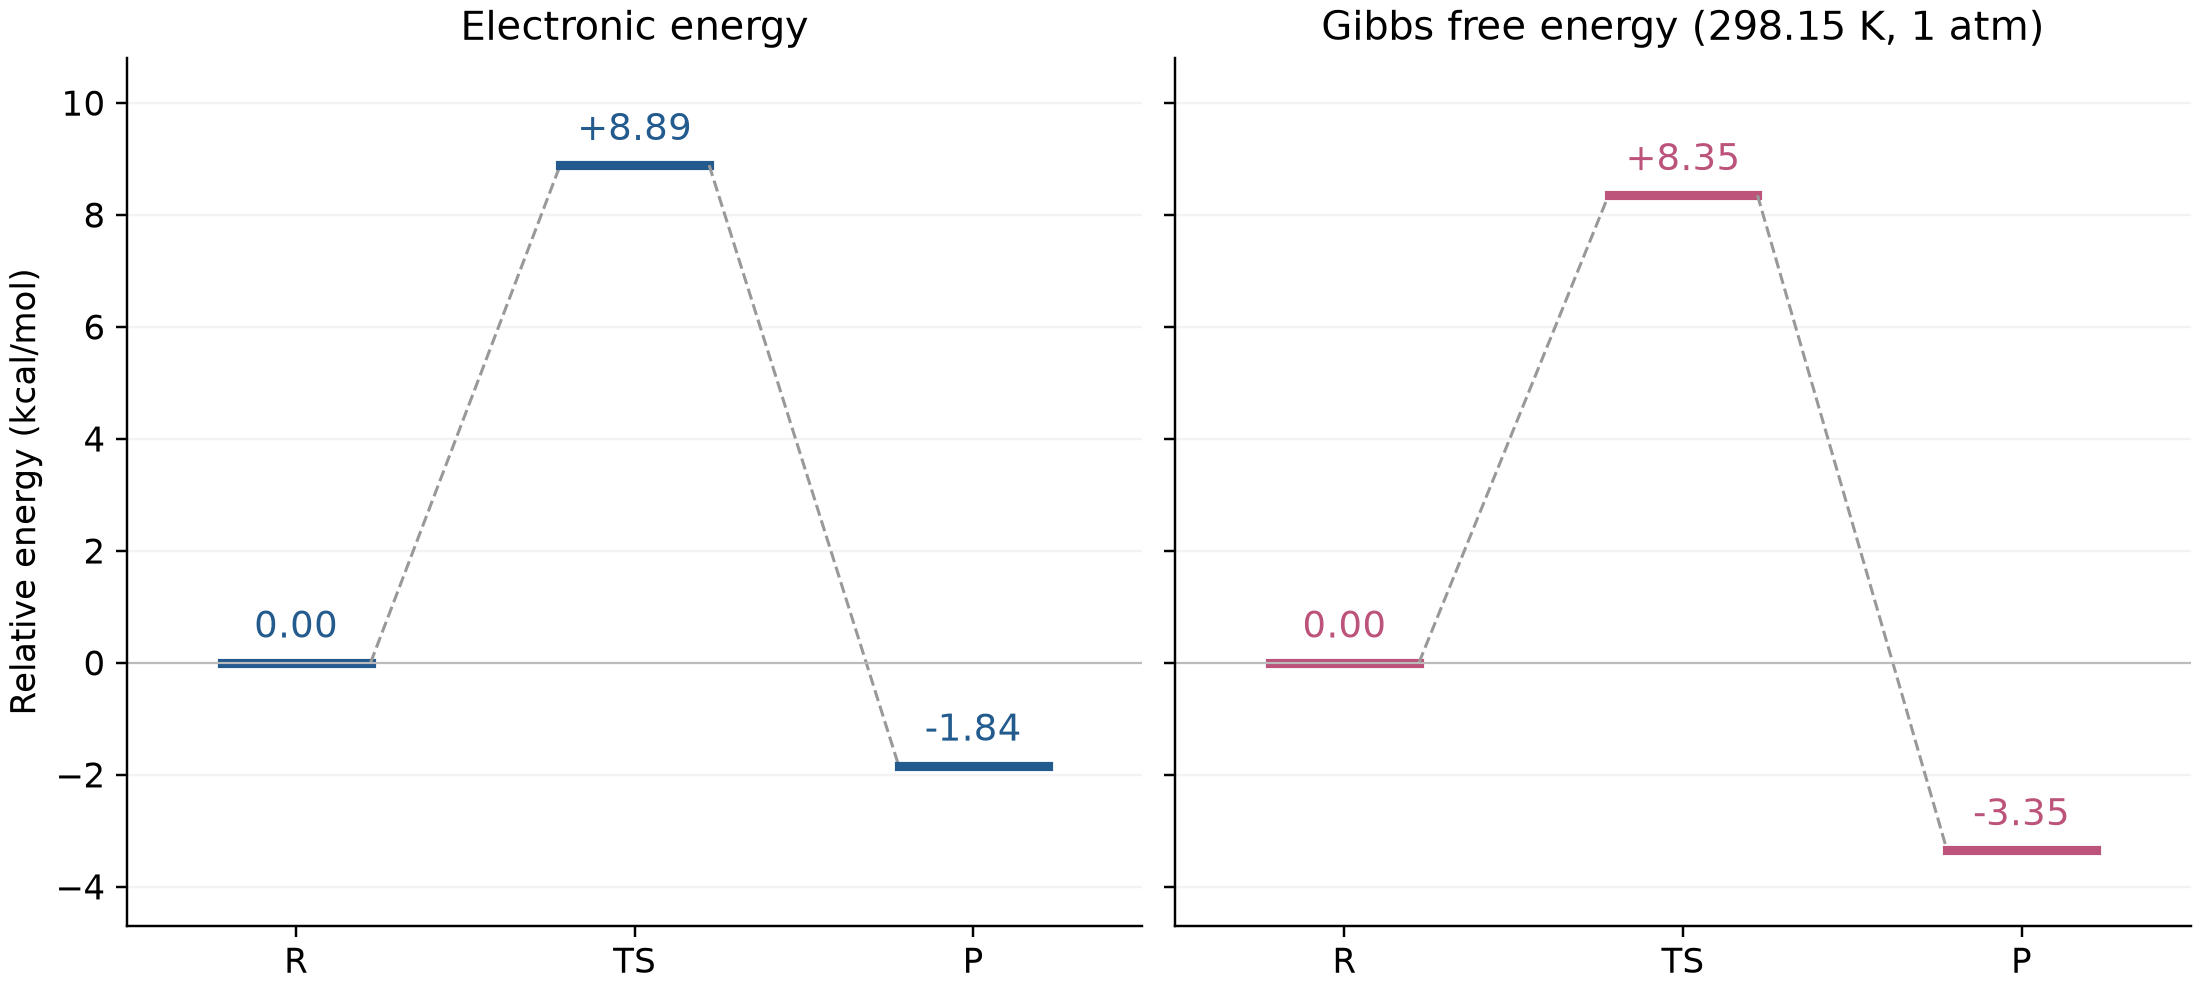
\includegraphics[width=\linewidth]{energy-gibbs-ladders.png}
\caption{离散驻点的电子能与 Gibbs 自由能阶梯图。
实线为驻点能级，虚线为示意连接；自由能采用 298.15 K、1 atm 的 RRHO 热校正。}
\end{figure}

\begin{table}[h!]
\centering\caption{相对能量与势垒（$\kcal$）}
\begin{tabular}{lrrrr}\toprule
过程 & $\Delta E$ & $\Delta(E+\mathrm{ZPE})$ & $\Delta H$ & $\Delta G$\\\midrule
R $\to$ TS & 8.89 & 8.11 & 7.84 & 8.35\\
R $\to$ P & $-1.84$ & $-2.65$ & $-2.23$ & $-3.35$\\
P $\to$ TS & 10.73 & 10.75 & 10.07 & 11.70\\\bottomrule
\end{tabular}
\end{table}

开环在电子能和自由能上均有利，但仍需越过有限势垒。
逆向自由能垒比正向高 $3.35\ \kcal$，与产物相对稳定程度一致。
这是单分子异构化，不需要双分子浓度标准态修正。

\subsection{零点能、热与熵的贡献}
将自由能差分解为
\begin{equation}
\Delta G=\Delta E+\Delta\mathrm{ZPE}
+\Delta(H-E-\mathrm{ZPE})-T\Delta S.
\end{equation}
正向电子势垒 $8.89\ \kcal$ 经零点能差降低 $0.78\ \kcal$，
其余焓热校正再降低 $0.26\ \kcal$，熵项则增加 $0.51\ \kcal$，
得到 $\Delta G^\ddagger=8.35\ \kcal$。
对应活化熵 $\Delta S^\ddagger=-1.70\ \mathrm{cal\,mol^{-1}K^{-1}}$。
反应熵为 $+3.77\ \mathrm{cal\,mol^{-1}K^{-1}}$，
$-T\Delta_{\rm r}S=-1.12\ \kcal$，进一步稳定开链产物。
\begin{figure}[htbp]
\centering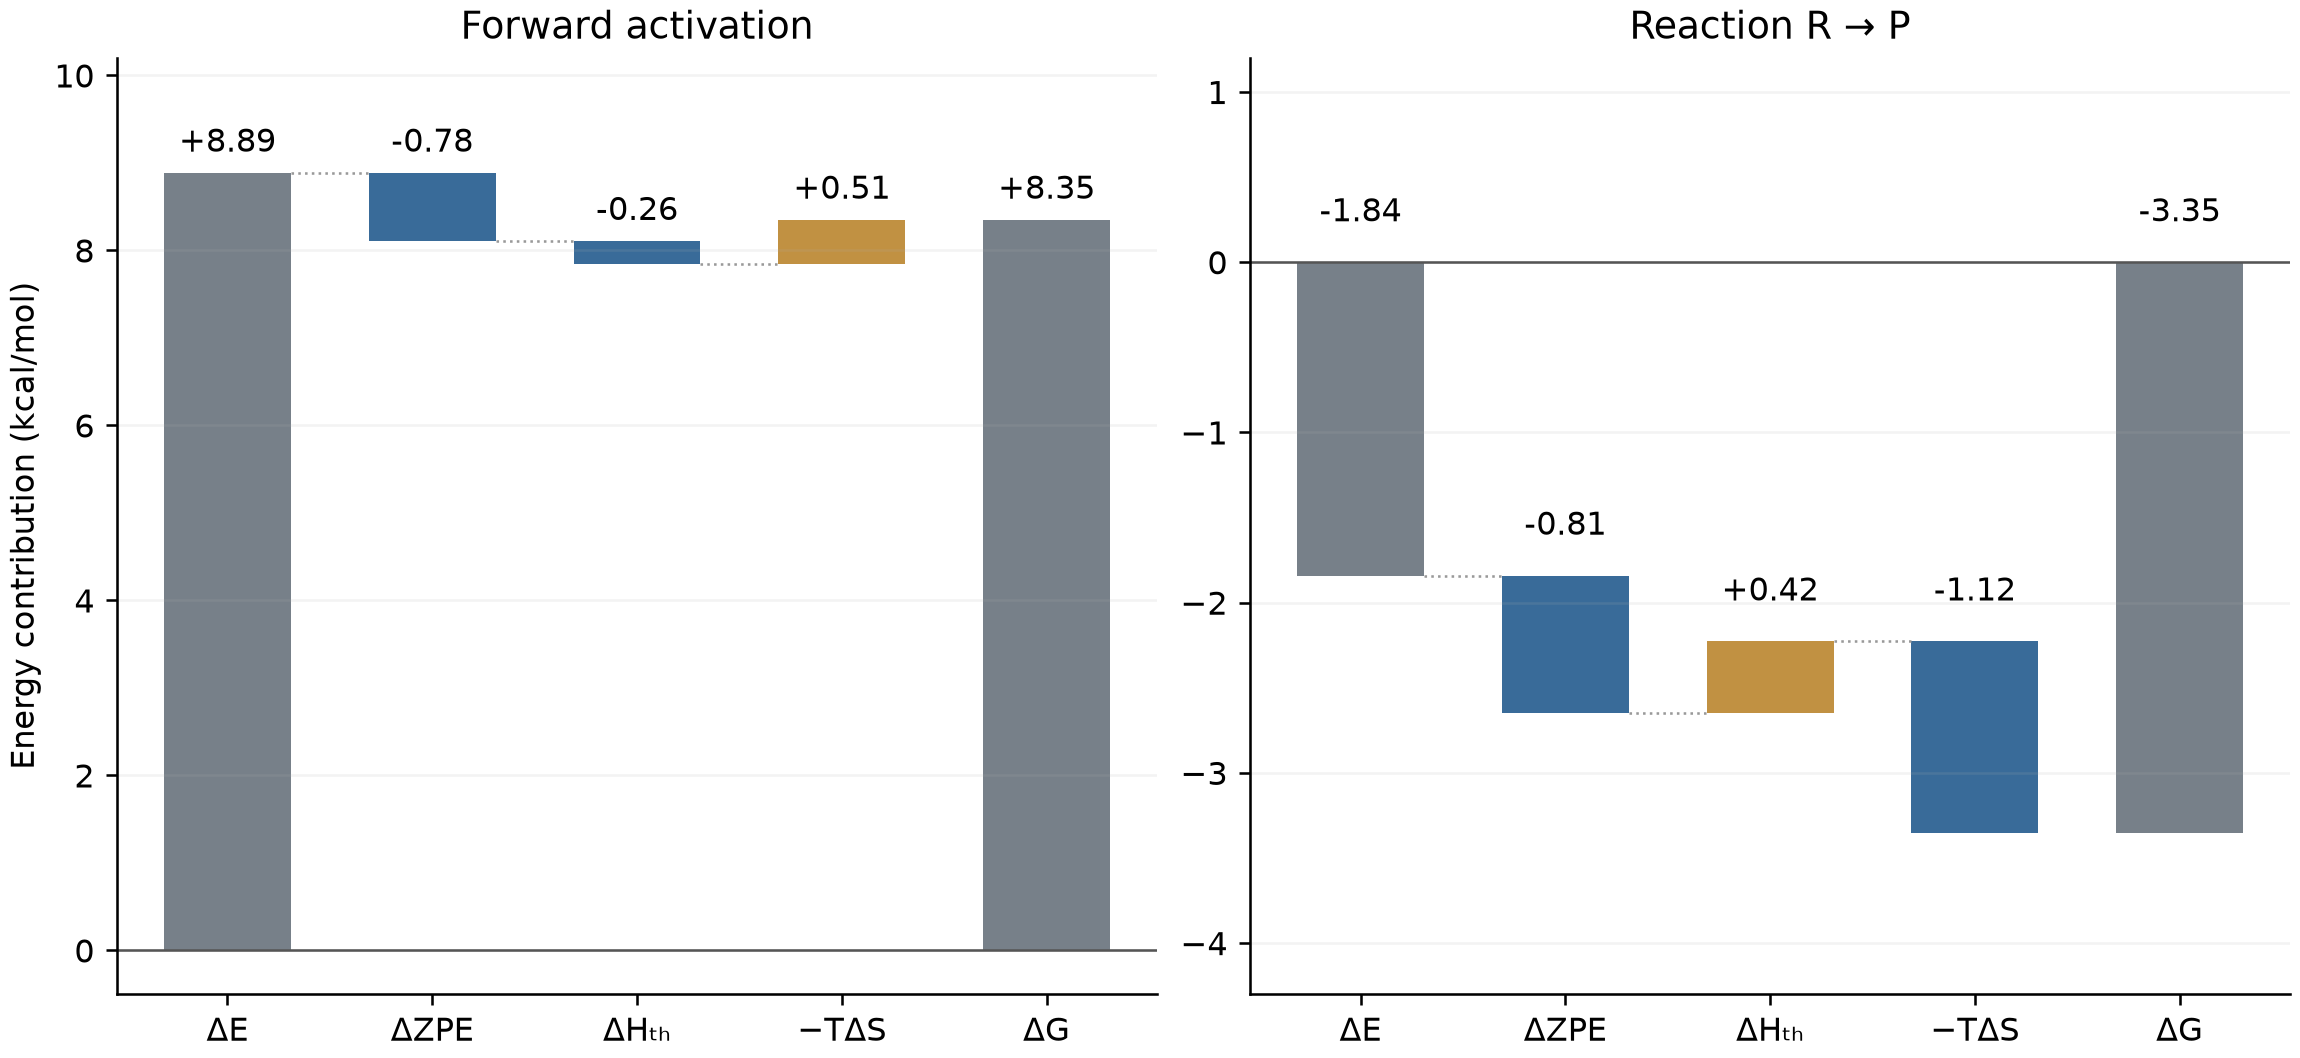
\includegraphics[width=\linewidth]{thermal-decomposition.png}
\caption{活化及反应自由能分解。$\Delta H_{\rm th}$ 为除电子能与 ZPE 以外的焓热校正。
灰色为起、终值，蓝色为降低自由能的贡献，金色为增加自由能的贡献；两图纵轴范围不同。}
\end{figure}
产物最低实频为 $98.79\ \mathrm{cm^{-1}}$，比环状反应物更软，
与开链结构具有较灵活的低频运动相符。RRHO 把这些运动视为谐振子，
熵因而对低频值较敏感。电子势垒和自由能势垒的差异，需要区分电子结构与低频热化学两类来源。

\subsection{固定几何下的基组与电子相关对照}
以各方法自己的反应物电子能为零点，得到表\ref{tab:methods}和图\ref{fig:methods}。
原 B3LYP-D3(BJ)/def2-SVP 的正向势垒为 $8.89\ \kcal$，
DLPNO-CCSD(T1)/def2-TZVPP 为 $8.94\ \kcal$，相差 $0.06\ \kcal$。

耦合簇反应电子能为 $-2.65\ \kcal$，比原 DFT 更有利 $0.81\ \kcal$。
其逆向势垒为 $11.59\ \kcal$。

\begin{table}[htbp]
\centering\small\caption{相同 R/TS/P 几何的电子能对照（$\kcal$）}\label{tab:methods}
\begin{tabular}{lrrr}\toprule
方法 / 基组 & 正向势垒 & 逆向势垒 & 反应能\\\midrule
B3LYP-D3(BJ) / def2-SVP & 8.89 & 10.73 & $-1.84$\\
B3LYP-D3(BJ) / def2-TZVPP & 7.42 & 11.01 & $-3.59$\\
M06-2X / def2-TZVPP & 12.41 & 11.44 & $+0.98$\\
DLPNO-CCSD(T1) / def2-TZVPP & 8.94 & 11.59 & $-2.65$\\\bottomrule
\end{tabular}
\end{table}

只将 B3LYP-D3(BJ) 的基组从 SVP 扩展为 TZVPP，正向势垒降低
$1.47\ \kcal$；在 TZVPP 下改用耦合簇，势垒又提高 $1.53\ \kcal$。
因此原小基组 DFT 与耦合簇势垒接近，包含基组变化和电子相关处理的部分抵消，
并不表示小基组效应本身很小。
M06-2X 的势垒比耦合簇高 $3.47\ \kcal$，反应电子能为 $+0.98\ \kcal$，
与其余三种结果的放能符号不同。
本体系的反应电子能仅数 $\kcal$，相对稳定性比“存在有限开环势垒”这一结论更敏感。

\begin{figure}[htbp]
\centering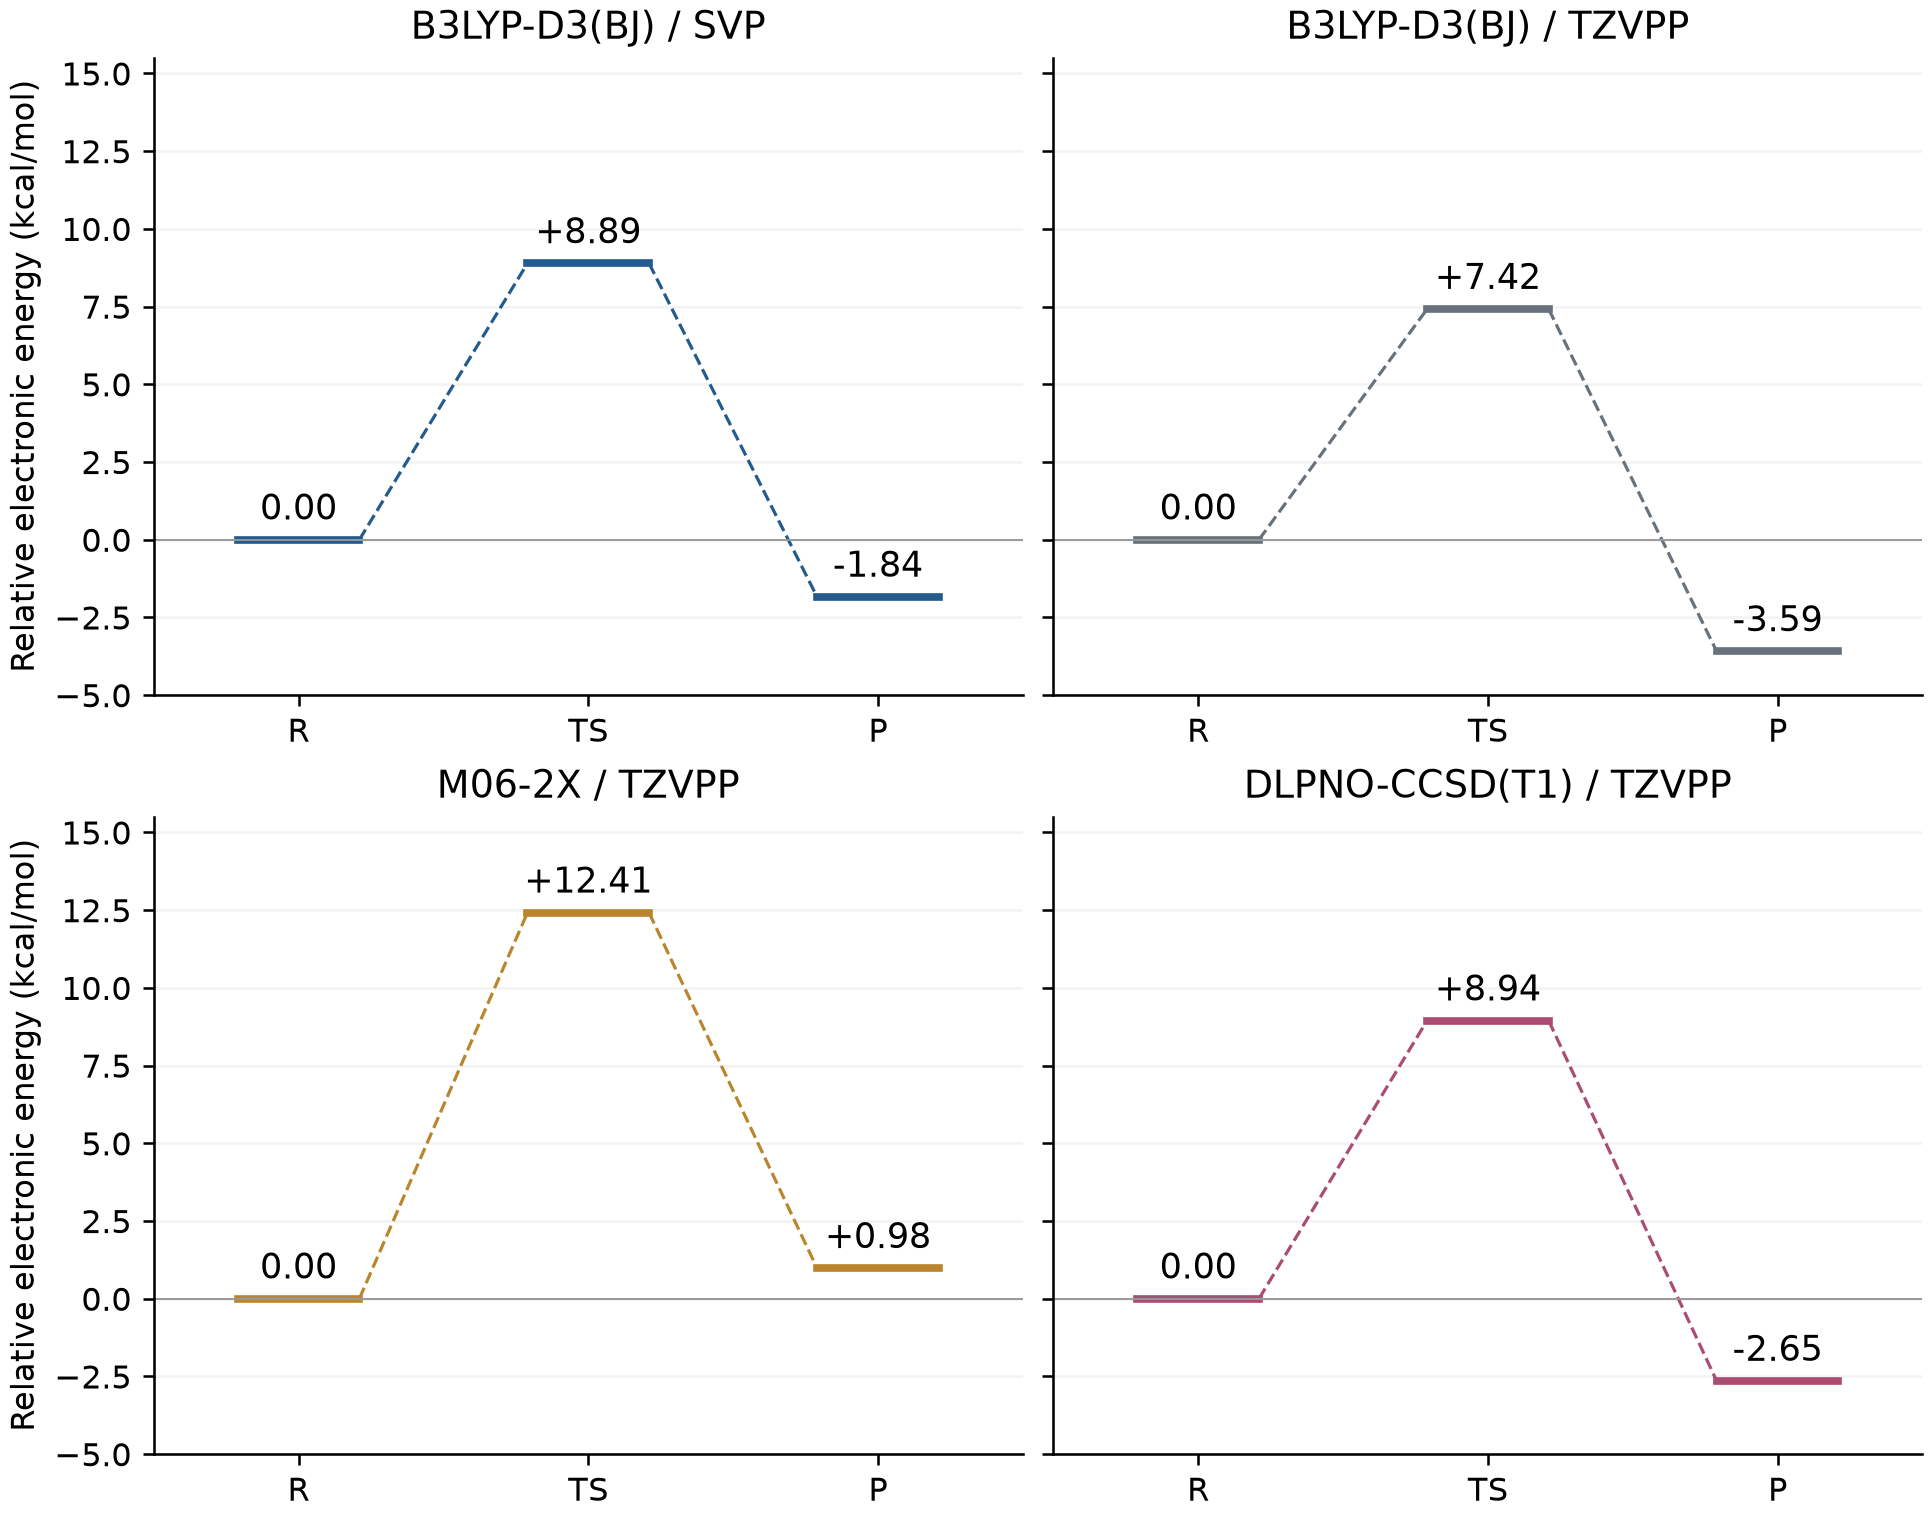
\includegraphics[width=\linewidth]{electronic-method-comparison.png}
\caption{四种电子能结果的离散能级图，使用相同纵轴和各方法独立的 R 零点。
全部几何来自 B3LYP-D3(BJ)/def2-SVP 驻点；虚线仅连接 R、TS、P 能级，不代表另算的 IRC。
三组单点不含新的零点能或热校正。}\label{fig:methods}
\end{figure}

\subsection{对照波函数与自旋布居}
两组 TZVPP 的 R/TS/P 波函数均通过稳定性检验，检验前后能量不变。
B3LYP-D3(BJ) 的 $\langle S^2\rangle$ 依次为 0.7550、0.7771、0.7541，
M06-2X 为 0.7564、0.7780、0.7554。
两种泛函均在 TS 处显示稍强的自旋污染，但没有发生多重度改变。

耦合簇的初始 UHF 值、相关波函数诊断列于表\ref{tab:ccdiag}。
TS 的 UHF $\langle S^2\rangle=0.958013$ 明显偏离双重态值 0.75；
实际耦合簇使用由其导出的 QRO，线性化 CCSD 诊断为 0.7531835，
$T_1=0.020537$，最大打印 PNO 振幅为 0.079153。
三态的 CCSD 与迭代三激发均收敛。
这些结果支持把耦合簇纳入电子能对照；初始 UHF 与线性化 CCSD 的
$\langle S^2\rangle$ 是不同层次的诊断，不作为严格自旋纯度或精确势垒的证明\cite{mdci}。

\begin{table}[htbp]
\centering\small\caption{开壳层耦合簇的参考与相关诊断}\label{tab:ccdiag}
\begin{tabular}{lrrr}\toprule
状态 & UHF $\langle S^2\rangle$ & 线性化 CCSD $\langle S^2\rangle$ & $T_1$ 诊断\\\midrule
R & 0.769233 & 0.7502617 & 0.013499\\
TS & 0.958013 & 0.7531835 & 0.020537\\
P & 0.774155 & 0.7501570 & 0.013111\\\bottomrule
\end{tabular}
\end{table}

对同一波函数进一步比较 Mulliken 与 Hirshfeld 原子自旋分配\cite{population}。
表\ref{tab:popcompare}中两种划分及两种泛函都给出 C9 $\to$ C1 的定位变化；
TS 的 C1、C9 共同承载自旋。
Hirshfeld 的碳原子数值较小，更多自旋分配给相邻原子；
Mulliken 的单个碳数值可超过 1，由其他原子的负自旋布居补偿。
所有完整 11 原子表的自旋总和均在 1 的 $2\times10^{-5}$ 以内，
电荷总和在零的同一容差以内。
因此自旋迁移方向对分区方法稳健，单原子数值则依赖分区定义。

\begin{table}[htbp]
\centering\small\caption{def2-TZVPP 下 C1、C9 的原子自旋布居}\label{tab:popcompare}
\begin{tabular}{llrrrr}\toprule
泛函 & 状态 & \multicolumn{2}{c}{Mulliken} & \multicolumn{2}{c}{Hirshfeld}\\
\cmidrule(lr){3-4}\cmidrule(lr){5-6}
 & & C1 & C9 & C1 & C9\\\midrule
B3LYP-D3(BJ) & R & 0.078 & 1.014 & 0.067 & 0.691\\
 & TS & 0.621 & 0.653 & 0.426 & 0.431\\
 & P & 1.063 & 0.005 & 0.748 & 0.004\\\midrule
M06-2X & R & 0.077 & 1.017 & 0.063 & 0.711\\
 & TS & 0.652 & 0.670 & 0.428 & 0.433\\
 & P & 1.060 & 0.002 & 0.763 & 0.004\\\bottomrule
\end{tabular}
\end{table}
\FloatBarrier

\subsection{文献热化学基准}
Cooksy 等采用 CCSD(T)/cc-pVTZ//QCISD/cc-pVDZ 研究同一反应，
在 298 K 报告 $\Delta G^\ddagger=8.49\ \kcal$、Arrhenius 活化能
$E_a=9.70\ \kcal$\cite{cooksy}。
本次活化自由能低 $0.14\ \kcal$，表明两种计算的势垒量级接近。
这一差值同时包含几何、基组、电子相关和热校正差异，不单独归为某个泛函的确定误差。
\begin{table}[htbp]
\centering\small\caption{同一开环反应的热化学文献对照（$\kcal$）}
\begin{tabular}{lrr}\toprule
计算 & $\Delta G^\ddagger$ & $E_a$\\\midrule
本次 UB3LYP-D3(BJ)/def2-SVP & 8.35 & 8.44\,$^{a}$\\
Cooksy 等 CCSD(T)//QCISD\cite{cooksy} & 8.49 & 9.70\\\bottomrule
\end{tabular}
\par\smallskip\raggedright\footnotesize
$^{a}$ 按经典过渡态理论局部关系 $E_a=\Delta H^\ddagger+RT$ 得到，
不是把电子势垒 $8.89$ 直接当作 Arrhenius 活化能。
\end{table}
PM7 约束扫描峰、无约束 DFT 的 $\Delta E^\ddagger$、文献 $E_a$ 和
$\Delta G^\ddagger$ 具有不同定义，必须同量比较。

\section{思考与讨论}
\subsection{为什么自由基开环能垒较低？}
三元环的几何约束带来环张力，开环后释放部分张力，同时 C2--C9 形成 $\pi$ 键。
TS 的 C1 和 C9 都承载显著自旋密度，说明未配对电子能够随骨架变化重新分布。
张力释放、双键形成和电子重新分布共同有利于较低能垒的开环。
但是反应并非无势垒：唯一开环负曲率、两侧下降的 IRC 和正的活化自由能共同表明存在明确的活化步骤。

\subsection{自旋极化、自旋污染和两个自由基是否等价？}
三者不等价。自旋极化是不同位置的 $\alpha$、$\beta$ 密度不平衡，
可以形成正负相间的布居；自旋污染描述非限制性波函数不是严格的 $\hat S^2$ 本征态。
TS 中两个碳都有较大自旋布居，不意味着体系变成两个独立自由基或另一种自旋态。
本次全程保持 31 电子双重态，积分自旋为 1，主要变化是同一未配对电子分布的位置。

\subsection{势垒能否直接给出实验速率？}
单分子过渡态理论为
\begin{equation}
k=\kappa\frac{k_{\rm B}T}{h}
\exp\!\left(-\frac{\Delta G^\ddagger}{RT}\right).
\end{equation}
该理论假定反应物达到热平衡，并与除去反应坐标的活化复合体保持准平衡；
透射系数 $\kappa$ 处理再穿越和量子动力学效应。
用本次 RRHO 自由能、取 $\kappa=1$，298.15 K 下单通道经典速率估计为
$4.70\times10^6\ \mathrm{s^{-1}}$。这是指定构象通道的理论估计，不是实验速率测定。

本反应已有重原子隧穿的直接证据：Gonzalez-James 等测得碳同位素动力学效应随降温增大，
加入小曲率隧穿的变分过渡态理论比半经典处理更好地再现实验结果\cite{tunneling}。
因此不能因为反应主要涉及碳原子，就认为隧穿必然可忽略。
本次频率和 IRC 确定势能通道，精确速率和同位素效应还需要相应动力学处理。

\section{结论}
在 UB3LYP-D3(BJ)/def2-SVP 水平上，环丙基甲基自由基经单一步骤开环。
TS 的 C1--C2 为 1.917 \AA、C2--C9 为 1.386 \AA，
唯一 $626.12i\ \mathrm{cm^{-1}}$ 模式对应断环与双键形成；
双向 IRC 与端点频率确认环状反应物及开链产物。

自旋布居与真实空间密度显示主要自旋由 C9 转移至 C1，
稳定性检验未改变所用波函数的能量。
电子活化能为 $8.89\ \kcal$，298.15 K、1 atm 下
$\Delta G^\ddagger=8.35\ \kcal$、$\Delta_{\rm r}G=-3.35\ \kcal$。
零点能降低活化势垒，开链产物还获得有利熵贡献。
固定相同几何的耦合簇电子势垒为 $8.94\ \kcal$，与原 DFT 相差 $0.06\ \kcal$；
基组扩展与电子相关处理对此接近值有部分抵消。
M06-2X 给出较高的 $12.41\ \kcal$ 及正的反应电子能，揭示了浅反应能的方法敏感性。
Mulliken 与 Hirshfeld 均确认相同的自旋迁移方向。
本次活化自由能与文献 $8.49\ \kcal$ 的结果量级一致。

\section*{数据与代码}
本实验的计算输入输出、图表、动画、复核脚本及报告源文件公开于：

\noindent\url{https://github.com/populuscathayana/Quantum4}

\clearpage
\begingroup\fontsize{10.5pt}{15pt}\selectfont
\begin{thebibliography}{99}
\bibitem{course} 浙江大学化学系. 自由基异构化反应的机理研究：量子化学实验课件. pp. 2--24.
\bibitem{irc} Gaussian, Inc. \textit{Gaussian 16 Keyword Reference: IRC}. 官方分销商文档. \url{https://www.conflex.co.jp/gaussian_support/irc.php}.
\bibitem{thermo} Ochterski, J. W. \textit{Thermochemistry in Gaussian}. Gaussian, Inc., 2000; updated 2022. \url{https://gaussian.com/wp-content/uploads/dl/thermo.pdf}.
\bibitem{m06} Zhao, Y.; Truhlar, D. G. The M06 suite of density functionals for main group thermochemistry, thermochemical kinetics, noncovalent interactions, excited states, and transition elements: two new functionals and systematic testing of four M06-class functionals and 12 other functionals. \textit{Theor. Chem. Acc.} \textbf{2008}, \textit{120}, 215--241. \url{https://doi.org/10.1007/s00214-007-0310-x}.
\bibitem{def2} Weigend, F.; Ahlrichs, R. Balanced basis sets of split valence, triple zeta valence and quadruple zeta valence quality for H to Rn: Design and assessment of accuracy. \textit{Phys. Chem. Chem. Phys.} \textbf{2005}, \textit{7}, 3297--3305. \url{https://doi.org/10.1039/B508541A}.
\bibitem{mdci} FACCTs; Max-Planck-Institut f\"ur Kohlenforschung. \textit{ORCA 6.1.1 Manual: Coupled Cluster and CI Theories (MDCI)}. \url{https://www.faccts.de/docs/orca/6.1/manual/contents/modelchemistries/mdci.html}.
\bibitem{opt} Gaussian, Inc. \textit{Gaussian 16 Keyword Reference: Opt}. 官方分销商文档. \url{https://www.conflex.co.jp/gaussian_support/opt.php}.
\bibitem{stable} Gaussian, Inc. \textit{Gaussian 16 Keyword Reference: Stable}. 官方分销商文档. \url{https://www.conflex.co.jp/gaussian_support/stable.php}.
\bibitem{population} Gaussian, Inc. \textit{Gaussian 16 Keyword Reference: Population}. 官方分销商文档. \url{https://www.conflex.co.jp/gaussian_support/population.php}.
\bibitem{cooksy} Cooksy, A. L.; King, H. F.; Richardson, W. H. Molecular Orbital Calculations of Ring Opening of the Isoelectronic Cyclopropylcarbinyl Radical, Cyclopropoxy Radical, and Cyclopropylaminium Radical Cation Series of Radical Clocks. \textit{J. Org. Chem.} \textbf{2003}, \textit{68}, 9441--9452. \url{https://doi.org/10.1021/jo035085b}.
\bibitem{tunneling} Gonzalez-James, O. M.; Zhang, X.; Datta, A.; Hrovat, D. A.; Borden, W. T.; Singleton, D. A. Experimental Evidence for Heavy-Atom Tunneling in the Ring-Opening of Cyclopropylcarbinyl Radical from Intramolecular $^{12}$C/$^{13}$C Kinetic Isotope Effects. \textit{J. Am. Chem. Soc.} \textbf{2010}, \textit{132}, 12548--12549. \url{https://doi.org/10.1021/ja1055593}.
\end{thebibliography}
\endgroup
\end{document}
